\chapter{Ein Schwarzes Loch erschaffen und das Rätsel am Horizont}

\lectureoverview{Wir werden ein Schwarzes Loch aus drei Bausteinen konstruieren: dem Kausaldiagramm der flachen Raumzeit, dem Schwarzschild-Diagramm und dem Satz von Birkhoff für eine sphärische Schale. Die Konstruktion zeigt, dass ein Ereignishorizont eine globale Grenze ist und in einem Bereich beginnen kann, der lokal noch flach ist. Anschließend wenden wir uns von der Kausalgeometrie der Entropie und der Hawking-Temperatur zu. Ein nahe am Horizont gehaltenes Thermometer wird beliebig heiß, während ein frei fallender Beobachter keinen lokalen Katastropheneffekt erwartet. Zum Abschluss wird gefragt, was ein Außenstehender durch ein Experiment tatsächlich feststellen kann, ohne dabei gerade die Störung hervorzurufen, die er nachweisen möchte.}

\section{Ein Schwarzes Loch bei der Temperatur des leeren Raums}

Eigentlich sollten Hausaufgaben aufgegeben worden sein: ein Schwarzes Loch bauen und es zum Vorzeigen und Besprechen in die Vorlesung mitbringen. Niemand hatte eines zum Vorzeigen, aber eine über Wolfram gefundene Rechnung lieferte eine einfachere Einstiegsfrage. Welchen Radius und welche Masse müsste ein Schwarzes Loch haben, damit seine Hawking-Temperatur nahe bei der \(3\,\mathrm{K}\) Temperatur der kosmischen Mikrowellenhintergrundstrahlung liegt?

\begin{classroomqa}
\audiencequestion{Was wurde auf der Website berechnet?\lecturetimestamp{00:00:39}}
\lecturerresponse{Der Radius eines Schwarzen Lochs, dessen Temperatur ungefähr \(3\,\mathrm{K}\) beträgt. Es geht nicht um eine präzise Rechnung, sondern um eine Abschätzung der physikalischen Größenordnung.}
\end{classroomqa}

Ein solches Loch hätte vorübergehend dieselbe Temperatur wie seine Umgebung, doch das Gleichgewicht wäre instabil. Ein Schwarzschild-Schwarzes-Loch hat eine negative Wärmekapazität. Wird es etwas heißer als das Wärmebad, strahlt es Energie ab, verliert Masse und wird noch heißer. Wird es etwas kälter, absorbiert es Energie, gewinnt Masse und wird noch kälter.\editorialnote{Das ist das präzise Stabilitätsargument hinter der bewusst groben Formulierung in der Vorlesung. Ein kanonisches Wärmebad kann für ein isoliertes Schwarzschild-Schwarzes-Loch kein stabiles Gleichgewicht herstellen.}

Die Abschätzung beginnt mit der charakteristischen Wellenlänge der Strahlung bei \(3\,\mathrm{K}\).

\begin{classroomqa}
\audiencequestion{Welche Wellenlänge hat Strahlung bei etwa drei Kelvin?\lecturetimestamp{00:02:03}}
\lecturerresponse{Im Hörsaal standen ein Zentimeter, \(21\) Zentimeter und sogar \(10\) Meter im Raum, bevor man sich auf den Mikrowellenbereich festlegte. Für die Argumentation genügte als brauchbare Größenordnung etwa ein Zentimeter – klein genug für die Scherze über einen Mikrowellenherd und einen Brotkasten.}
\end{classroomqa}

Das typische Hawking-Quant hat, bis auf numerische Faktoren, eine Wellenlänge in der Größenordnung des Schwarzschild-Radius:
\begin{equation}
\lambda_{\mathrm{H}}\sim R_s,
\qquad
R_s=\frac{2GM}{c^2}.
\label{eq:l05-scale}
\end{equation}
Setzt man den in der Vorlesung verwendeten Wert \(\lambda_{\mathrm H}\sim1\,\mathrm{cm}\) ein, erhält man \(R_s\sim1\,\mathrm{cm}\). Da ein Schwarzes Loch mit Sonnenmasse einen Radius von einigen Kilometern hat und \(R_s\) proportional zu \(M\) ist, ergibt sich für die entsprechende Masse ungefähr
\begin{equation}
M\sim10^{-5}M_\odot,
\label{eq:l05-rough-mass}
\end{equation}
also eine planetare Größenordnung. Daher kommt die Vorlesung auf eine erdähnliche Abschätzung.

\begin{classroomqa}
\audiencequestion{Stimmt das mit dem Zahlenwert von Wolfram überein?\lecturetimestamp{00:05:53}}
\lecturerresponse{Der angegebene Wert lag näher an der Mondmasse. Das schien im Vergleich zur groben Abschätzung klein, doch beide Werte verdeutlichen den entscheidenden Punkt: Ein solches Objekt kann man nicht in der Tasche tragen.}
\end{classroomqa}

Wenn man die Konstanten beibehält, wird die Abweichung verständlich. Aus
\begin{equation}
T_H=\frac{\hbar c}{4\pi k_B R_s},
\end{equation}
erhält man für \(T_H=3\,\mathrm{K}\)
\begin{equation}
R_s\simeq6.1\times10^{-5}\,\mathrm{m},
\qquad
M\simeq4.1\times10^{22}\,\mathrm{kg}.
\label{eq:l05-three-kelvin}
\end{equation}
Das entspricht eher der Mond- als der Erdmasse. Die Mikrowellen-Wellenlänge, der Faktor \(4\pi\) und die Wahl der typischen Wellenlänge eines Schwarzkörpers erklären den Unterschied zwischen der schnellen Abschätzung und dem Zahlenwert.\editorialnote{Gleichung~\eqref{eq:l05-three-kelvin} enthält wieder die numerischen Faktoren, die in der Dimensionsabschätzung der Vorlesung weggelassen wurden. Die Abschätzung selbst bleibt erhalten, denn so wurde in der Vorlesung vorgegangen.}

Die Rechnung hat ihren Zweck erfüllt. Jetzt wollen wir ein Schwarzes Loch mathematisch und gedanklich konstruieren. Die vollständigen Feldgleichungen sind für den vorliegenden Zweck zu schwierig. Die grundlegenden Tatsachen lassen sich anhand von Bildern darstellen.

\section{Der erste Baustein: flache Raumzeit}

Wir verwenden Polarkoordinaten mit Ursprung beim Beobachter und unterdrücken die Winkelkoordinaten. Die reduzierten Koordinaten sind \((t,r)\) mit \(r\geq0\). Ein Punkt in diesem reduzierten Diagramm ist kein Punkt der vierdimensionalen Raumzeit; außer bei \(r=0\) steht er für eine ganze Zweikugel \(S^2\).

Radiale Lichtstrahlen bewegen sich unter einem Winkel von \(45^\circ\). Ein einlaufender Strahl erreicht den Ursprung, ein auslaufender verlässt ihn entlang der anderen Nullrichtung. Die unendliche Halbebene lässt sich durch eine konforme Transformation zu einem endlichen Penrose-Keil komprimieren. Diese Transformation ist nicht eindeutig. Entscheidend ist, dass sie das Unendliche auf eine endliche Grenze abbildet und die radialen Nullrichtungen bei \(45^\circ\) belässt. In der Sprache der Tafel: Wir stauchen das Diagramm zusammen.

\begin{figure}[htbp]
\centering
\includegraphics[width=0.68\textwidth]{lecture_05_figure_02.png}
\caption{Die obere Hälfte der kompaktifizierten radialen Minkowski-Raumzeit. Die vertikale Kante ist \(r=0\), während sich die Kurvenscharen zum kompaktifizierten Unendlichen hin verdichten.}
\lectureframe{00:11:41.560}
\end{figure}

\begin{figure}[htbp]
\centering
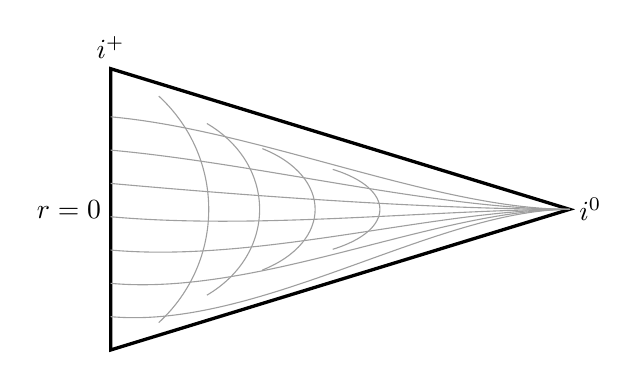
\begin{tikzpicture}[scale=0.94]
\coordinate (O) at (0,0);
\coordinate (P) at (0,3.8);
\coordinate (I) at (6.2,1.9);
\draw[very thick] (O)--(P)--(I)--cycle;
\foreach \y in {0.45,0.90,1.35,1.80,2.25,2.70,3.15} {
  \draw[gray!75] (0,\y) .. controls (2.0,\y-0.18) and (4.4,1.9) .. (I);
}
\draw[gray!75] (0.65,0.37) .. controls (1.55,1.20) and (1.55,2.60) .. (0.65,3.43);
\draw[gray!75] (1.30,0.74) .. controls (2.25,1.30) and (2.25,2.50) .. (1.30,3.06);
\draw[gray!75] (2.05,1.08) .. controls (3.00,1.46) and (3.00,2.34) .. (2.05,2.72);
\draw[gray!75] (3.00,1.36) .. controls (3.85,1.62) and (3.85,2.18) .. (3.00,2.44);
\node[left] at (0,1.9) {\(r=0\)};
\node[above] at (P) {\(i^+\)};
\node[right] at (I) {\(i^0\)};
\end{tikzpicture}
\caption{Eine übersichtliche Fassung des oberen Keils. Die Kurven stellen qualitative Familien mit konstantem \(r\) und konstantem \(t\) dar, kein exaktes Koordinatennetz.}
\label{fig:l05-flat-wedge}
\end{figure}

Weltlinien bei konstantem \(r\) verlaufen vor der Kompaktifizierung vertikal, krümmen sich dann aber und häufen sich nahe dem zukünftigen zeitartigen Unendlichen. Auch die Schnitte mit konstantem \(t\) verdichten sich zum räumlichen Unendlichen hin. Diese Verdichtung ist ein Koordinateneffekt, keine physikalische Kompression von Materie.

Die \(45^\circ\)-Regel gilt unmittelbar für radiales Licht. Ein Strahl mit Drehimpuls kann den Ursprung verfehlen, einen von null verschiedenen kleinsten Abstand erreichen und anschließend wieder nach außen laufen. Weit vom Ursprung entfernt sieht seine projizierte Bewegung fast radial aus; erst nahe dem kleinsten Abstand krümmt sich die reduzierte \((t,r)\)-Bahn sichtbar. Damit ist der erste Baustein abgeschlossen.

\section{Der zweite Baustein: die ewige Schwarzschild-Raumzeit}

Die maximal fortgesetzte Schwarzschild-Lösung hat zwei äußere Diamanten, einen zukünftigen Schwarzen-Loch-Bereich und einen vergangenen Weiß-Loch-Bereich. Ihre obere und untere wellenförmige Grenze sind die zukünftige beziehungsweise vergangene Singularität. Für ein durch Kollaps entstandenes Schwarzes Loch werden wir den größten Teil dieser Struktur bald verwerfen; der gewöhnliche rechte Außenbereich ist jedoch genau der Teil, den wir benötigen.

\begin{figure}[htbp]
\centering
\includegraphics[width=0.72\textwidth]{lecture_05_figure_03.png}
\caption{Das ewige Schwarzschild-Diagramm mit dem gewöhnlichen Außenbereich und seinem schematischen Koordinatennetz auf der rechten Seite.}
\lectureframe{00:16:55.975}
\end{figure}

\begin{figure}[htbp]
\centering
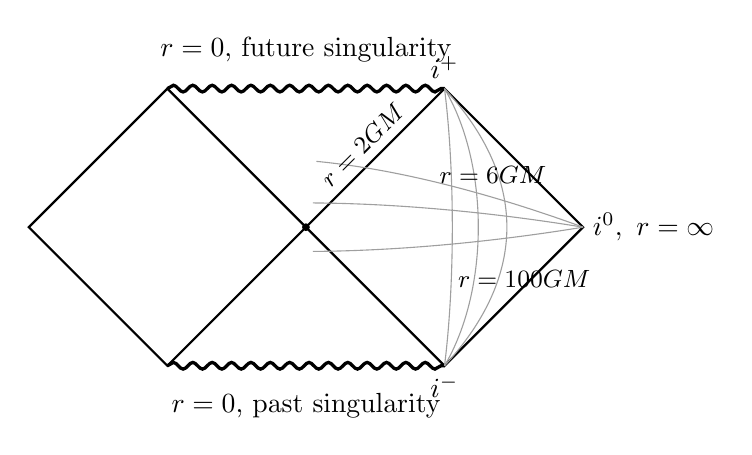
\begin{tikzpicture}[scale=0.88]
\coordinate (C) at (0,0);
\coordinate (TL) at (-2.0,2.0);
\coordinate (L) at (-4.0,0);
\coordinate (BL) at (-2.0,-2.0);
\coordinate (TR) at (2.0,2.0);
\coordinate (R) at (4.0,0);
\coordinate (BR) at (2.0,-2.0);
\draw[thick] (C)--(TL)--(L)--(BL)--(C);
\draw[thick] (C)--(TR)--(R)--(BR)--(C);
\draw[very thick,decorate,decoration={snake,amplitude=1.2pt,segment length=7pt}] (TL)--(TR);
\draw[very thick,decorate,decoration={snake,amplitude=1.2pt,segment length=7pt}] (BL)--(BR);
\draw[gray!75] (TR) .. controls (2.15,0.8) and (2.15,-0.8) .. (BR);
\draw[gray!75] (TR) .. controls (2.65,0.9) and (2.65,-0.9) .. (BR);
\draw[gray!75] (TR) .. controls (3.20,0.7) and (3.20,-0.7) .. (BR);
\draw[gray!75] (0.15,0.95) .. controls (1.5,0.82) and (2.9,0.40) .. (R);
\draw[gray!75] (0.10,0.35) .. controls (1.5,0.34) and (2.9,0.18) .. (R);
\draw[gray!75] (0.10,-0.35) .. controls (1.5,-0.34) and (2.9,-0.18) .. (R);
\fill (C) circle (1.6pt);
\node[above] at (TR) {\(i^+\)};
\node[below] at (BR) {\(i^-\)};
\node[right] at (R) {\(i^0,\ r=\infty\)};
\node[above] at (0,2.25) {\(r=0\), future singularity};
\node[below] at (0,-2.25) {\(r=0\), past singularity};
\node[rotate=45,above,font=\small] at (1.0,1.0) {\(r=2GM\)};
\node[font=\small] at (2.70,0.75) {\(r=6GM\)};
\node[font=\small] at (3.15,-0.75) {\(r=100GM\)};
\end{tikzpicture}
\caption{Der rechte Außenbereich ähnelt bei großen Radien dem flachen Keil. Seine innere Nullkante liegt bei \(r=2GM\), wenn \(c=1\); die übrigen eingezeichneten Radien sind schematische Beispiele.}
\label{fig:l05-eternal-schwarzschild}
\end{figure}

Weit vom Loch entfernt ähnelt der Außenbereich immer stärker dem kompaktifizierten flachen Raum. Linien wie \(r=6GM\) und \(r=100GM\) nähern sich dem Verlauf gewöhnlicher Weltlinien mit konstantem Radius an. Die innere Grenze des Außenbereichs liegt bei
\begin{equation}
r=2GM
\end{equation}
in Einheiten mit \(c=1\).

Nahe dem Zentrum scheitert der Vergleich mit dem flachen Raum. Ein radialer Strahl in der Minkowski-Raumzeit erreicht \(r=0\) und tritt auf der gegenüberliegenden physikalischen Seite wieder aus. Ein zukunftsgerichteter Strahl im Inneren der Schwarzschild-Raumzeit prallt nicht zurück. Er endet an der raumartigen Singularität bei \(r=0\). Diesen kausalen Unterschied muss die Konstruktion des Kollaps bewahren.

\section{Der Satz, mit dem sich die Bausteine verbinden lassen}

Das fehlende Element taucht zuerst in der Newtonschen Gravitation auf. Für eine kugelsymmetrische Massenverteilung ergibt das Gaußsche Gesetz
\begin{equation}
\oint\mathbf g\cdot d\mathbf A=-4\pi G M_{\mathrm{enc}},
\end{equation}
und damit
\begin{equation}
\mathbf g(r)=-\frac{G M_{\mathrm{enc}}(r)}{r^2}\,\hat{\mathbf r}.
\label{eq:l05-shell-theorem}
\end{equation}
Materie außerhalb der Kugel mit Radius \(r\) trägt dort nicht zum resultierenden Feld bei. Für eine hohle Schale mit Gesamtmasse \(M\) gilt
\begin{equation}
\mathbf g=
\begin{cases}
0, & r<R_{\mathrm{shell}},\\[3pt]
-\dfrac{GM}{r^2}\hat{\mathbf r}, & r>R_{\mathrm{shell}}.
\end{cases}
\end{equation}

Der Satz von Birkhoff ist das relativistische Gegenstück. Jeder kugelsymmetrische Vakuumbereich ist lokal ein Schwarzschild-Bereich mit einem konstanten Massenparameter. Der leere Innenraum einer kugelförmigen Schale hat den Massenparameter null und ist lokal Minkowski; außen beträgt der Massenparameter \(M\), und der Bereich ist Schwarzschild:
\begin{equation}
\begin{aligned}
M_{\mathrm{enc}}&=0 && \text{inside the shell},\\
M_{\mathrm{enc}}&=M && \text{outside the shell}.
\end{aligned}
\label{eq:l05-birkhoff}
\end{equation}
Die Aussage bleibt auch dann nützlich, wenn sich die Schale bewegt, denn die Vakuumbereiche auf beiden Seiten bleiben kugelsymmetrisch.

\editorialnote{„Innen flach“ ist eine lokale Aussage. Eine statische Schale kann die Normierung der inneren Zeitkoordinate verändern, obwohl die Krümmung im Inneren verschwindet. Bei einer bewegten oder lichtartigen Schale müssen die beiden Vakuummetriken über die Schale hinweg angepasst werden; die idealisierte Konstruktion ist eine Dünnschalenverklebung, die eng mit der einlaufenden Vaidya-Geometrie verwandt ist. Keine dieser Einschränkungen ändert das hier verwendete kausale Ausschneide- und Einfügeargument.}

Für eine anschauliche Vorstellung im Labor denke man an eine Kugel, die dicht mit synchronisierten Lasern bedeckt ist, wie in einer großen Anlage zur Trägheitsfusion. Alle Laser werden gleichzeitig nach innen gerichtet ausgelöst. In der Idealisierung gibt es keinen Apparat, sondern nur eine perfekt kugelförmige Lichtschale. Die Schale trägt die Energie \(E\), sodass der äußere Massenparameter
\begin{equation}
M=\frac{E}{c^2},
\end{equation}
beträgt, oder in natürlichen Einheiten einfach \(E=M\). Da sich die Schale mit Lichtgeschwindigkeit bewegt, entspricht sie im reduzierten Diagramm einer einlaufenden Nullinie. Jeder Punkt auf dieser Linie steht für eine vollständige kugelförmige Wellenfront, nicht für die Bahn eines einzelnen Photons.

\section{Die Raumzeit des Kollapses zusammensetzen}

Wir beginnen mit der flachen Raumzeit und zeichnen die einlaufende Nullschale ein. Der Bereich innerhalb der Schale ist korrekt: Nach dem Satz von Birkhoff ist er flach. Der Außenbereich ist falsch, denn seine Schwarzschild-Geometrie muss bereits die Gesamtmasse der Schale berücksichtigen.

Nun zeichnen wir dieselbe Schale im ewigen Schwarzschild-Diagramm ein. Dort ist der Bereich außerhalb der Schale korrekt. Das Weißloch, der zweite Außenbereich und der für einen Kollaps aus gewöhnlichem leerem Raum unpassende Teil des Inneren des Schwarzen Lochs sind falsch, also löschen wir sie.

\begin{figure}[htbp]
\centering
\includegraphics[width=0.72\textwidth]{lecture_05_figure_05.png}
\caption{Die rot eingezeichnete Nullschale im Schwarzschild-Diagramm, während der passende Außenbereich herausgelöst wird.}
\lectureframe{00:32:00.000}
\end{figure}

Im flachen Teil erreicht die Schale \(r=0\). Im Schwarzschild-Teil erreicht sie den Anfang der zukünftigen Singularität. Das ist derselbe Endpunkt. Verklebt man das flache Innere entlang der Schale mit dem Schwarzschild-Außenbereich, erhält man die einfachste Raumzeit für die Entstehung eines Schwarzen Lochs.

\begin{classroomqa}
\audiencequestion{Ist am Verbindungspunkt links oben der Endpunkt im flachen Raum wirklich derselbe Punkt wie auf der Schwarzschild-Seite?\lecturetimestamp{00:34:50}}
\lecturerresponse{Ja. Die flache Lichtschale zieht sich bis auf \(r=0\) zusammen, und auch die Schwarzschild-Singularität liegt bei \(r=0\). Die beiden identifizierten Punkte haben dieselbe geometrische Bedeutung: Die Zweikugel ist auf null Größe geschrumpft.}
\end{classroomqa}

\begin{figure}[htbp]
\centering
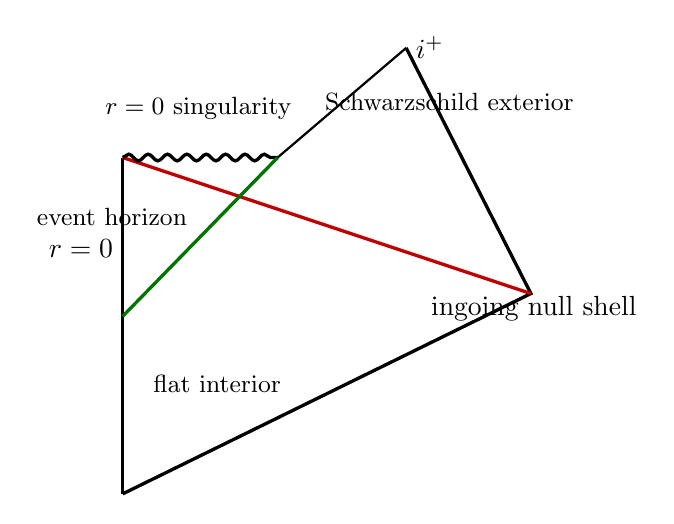
\begin{tikzpicture}[scale=0.96]
\coordinate (A) at (0,-2.8);
\coordinate (B) at (0,1.65);
\coordinate (C) at (2.05,1.65);
\coordinate (D) at (5.4,-0.15);
\coordinate (E) at (3.75,3.10);
\coordinate (H0) at (0,-0.45);
\draw[very thick] (A)--(B);
\draw[very thick] (A)--(D)--(E);
\draw[very thick,red!75!black] (D)--(B);
\draw[very thick,decorate,decoration={snake,amplitude=1.2pt,segment length=7pt}] (B)--(C);
\draw[very thick,green!45!black] (H0)--(C);
\draw[thick] (C)--(E);
\node[left] at (0,0.45) {\(r=0\)};
\node[below right] at (3.95,-0.05) {ingoing null shell};
\node[font=\small] at (1.25,-1.35) {flat interior};
\node[font=\small,anchor=west] at (2.55,2.38) {Schwarzschild exterior};
\node[above,font=\small] at (1.0,2.02) {\(r=0\) singularity};
\node[above left,font=\small] at (0.98,0.62) {event horizon};
\node[right] at (E) {\(i^+\)};
\end{tikzpicture}
\caption{Die Kollapsgeometrie. Die rote Schale verbindet ein flaches Inneres mit einem Schwarzschild-Außenbereich. Der grüne Ereignishorizont beginnt früher im flachen Bereich und endet an der zukünftigen Grenze des Schwarzen-Loch-Bereichs.}
\label{fig:l05-collapse}
\end{figure}

Diese Konstruktion beantwortet eine offene Frage zur ewigen Lösung. Ein durch Kollaps entstandenes Schwarzes Loch hat weder ein vergangenes Weißloch noch ein zweites asymptotisches Universum. Eine zukünftige Singularität hat es dennoch.

\section{Der Horizont ist eine globale Grenze}

Die frühere Bezeichnung \(r=2GM\) kennzeichnete den Horizont in der stationären Schwarzschild-Geometrie, ist aber nicht die Definition, die man in einer dynamischen Raumzeit benötigt.

\begin{definition}Der zukünftige Ereignishorizont ist die Grenze der Menge aller Ereignisse, von denen aus ein zukunftsgerichtetes kausales Signal die zukünftige Nullunendlichkeit erreichen kann.
\end{definition}

Im Kollapsdiagramm verfolgt man den auslaufenden Nullstrahl, dem die Flucht gerade misslingt. Strahlen knapp außerhalb erreichen das Unendliche; Strahlen knapp innerhalb enden an der Singularität. Diese Trennlinie ist der wirkliche Horizont.

\begin{figure}[htbp]
\centering
\includegraphics[width=0.72\textwidth]{lecture_05_figure_06.png}
\caption{Die fertige Konstruktion an der Tafel. Die einlaufende Schale ist rot, der Ereignishorizont grün; ein Teil der grünen Linie liegt unterhalb der Schale im noch flachen Bereich.}
\lectureframe{00:39:10.000}
\end{figure}

Das verblüffende Merkmal lässt sich nun nicht mehr übersehen. Der Horizont reicht rückwärts in einen Bereich, den die Schale noch nicht erreicht hat. Die Geometrie ist dort lokal flach, und ein Beobachter, der diese Linie überquert, stellt weder einen Krümmungsimpuls noch eine Wand oder einen Lichtblitz fest. Trotzdem kann der Beobachter das Unendliche bereits nicht mehr erreichen, weil die zukünftige Schale alle möglichen Fluchtwege versperren wird. Ereignishorizonte sind genau in diesem globalen Sinn teleologisch: Um einen solchen Horizont zu lokalisieren, muss man die gesamte Zukunft der Raumzeit kennen.\editorialnote{Kein lokales Experiment kann feststellen, dass gerade ein glatter Ereignishorizont überquert wurde. Andere Begriffe wie scheinbare oder gefangene Horizonte sind lokaler und müssen beim Kollaps nicht mit dem Ereignishorizont zusammenfallen.}

Die Analogie mit dem Abfluss veranschaulicht den kausalen Gedanken. Man stelle sich einen Ruderer in einem stillen See nahe einem verstopften Abfluss vor. Bliebe der Stöpsel für immer an Ort und Stelle, könnte der Ruderer entkommen. Ist jedoch sicher, dass ihn jemand herausziehen wird, kann die spätere Strömung die Flucht unmöglich machen, obwohl sich das Wasser noch nicht bewegt. Ein gefrorener Niagarafall veranschaulicht denselben Punkt: Ruhiges Wasser garantiert keinen sicheren Fluchtweg in der Zukunft.

\begin{classroomqa}
\audiencequestion{Wird der Stöpsel gezogen, weil sich die kugelförmige Lichtschale immer stärker konzentriert?\lecturetimestamp{00:43:13}}
\lecturerresponse{Die Konzentration lässt das Schwarze Loch entstehen. Die Abflussgeschichte soll jedoch einen enger gefassten Punkt veranschaulichen: Man kann bereits hinter dem Punkt ohne Wiederkehr sein, bevor lokal etwas Dramatisches geschieht.}
\end{classroomqa}

\subsection{Ein Horizont aus wachsenden Kugeln}

Jeder Punkt des reduzierten Horizonts steht für eine \(S^2\). Am ersten Punkt des Horizonts hat diese Kugel eine Fläche von null. Geht man entlang des Horizonts nach oben, wächst die Kugel, bis ihr Flächenradius
\begin{equation}
R_s=\frac{2GM}{c^2}.
\end{equation}
erreicht. Bei einem stationären Loch behält sie diese Größe; fällt weitere Energie hinein, wächst sie erneut.

\editorialnote{Im idealisierten Diagramm des kugelsymmetrischen Kollapses treffen die Erzeugenden des Horizonts in einem Entstehungspunkt, auch Knickpunkt genannt, auf \(r=0\) zusammen. Diese Grenz-Zweikugel hat eine Fläche von null; die Aussage ist nicht so zu verstehen, als schrumpfe ein endlicher Schwarzschild-Horizont plötzlich zu einem Punkt.}

\subsection{Was der weit entfernte Beobachter rekonstruieren kann}

Die folgende ausführliche Erörterung unterscheidet zwischen einem Beobachter, der sich bereits innerhalb des globalen Horizonts befindet, und der Geschichte, durch die er dorthin gelangt ist.

\begin{classroomqa}
\audiencequestion{Was ist mit der Person, die gefangen ist, bevor die Schale eintrifft? Befindet sie sich aus Sicht des weit entfernten Beobachters außerhalb des Horizonts?\lecturetimestamp{00:44:03}}
\lecturerresponse{Nein. Sobald die Weltlinie hinter dem Ereignishorizont liegt, erreicht sie in der Zukunft die Singularität, und kein neues Signal von dort erreicht den weit entfernten Beobachter. Die Person ist jedoch nicht erst dort entstanden. Frühere Teilchen, Vorläufer oder andere Vorläuferenergie sind aus einem sichtbaren Bereich hineingelangt.}
\end{classroomqa}

Der weit entfernte Beobachter kann also die Vorläufermaterie auf den Horizont zukommen sehen, ohne jemals ein Signal von dessen Innerem zu empfangen. Es ist kein Widerspruch, durch die einlaufende Schale hindurchzusehen: Sie besteht aus Licht, und der Beobachter kann auch die Schale selbst sehen und daraus schließen, dass ein Schwarzes Loch entstanden ist.

\begin{classroomqa}
\audiencequestion{Verläuft die Sichtlinie durch die kollabierende Schale, und kann der Außenbeobachter trotzdem erkennen, dass das Loch entstanden ist?\lecturetimestamp{00:46:51}}
\lecturerresponse{Ja. Der Beobachter sieht die einlaufende Schale und kann Licht empfangen, dessen Weg sie kreuzt, solange dieses Licht noch entkommen kann. Seltsam wirkt, dass sich die Vorläufermaterie dem soeben festgelegten Horizont nähert, noch bevor die Schale das Zentrum erreicht.}
\end{classroomqa}

\begin{classroomqa}
\audiencequestion{Gilt damit weiterhin die Vorstellung, dass Materie für einen Außenstehenden so aussieht, als werde sie auf den Horizont zusammengedrückt?\lecturetimestamp{00:47:49}}
\lecturerresponse{Ja. In der Beschreibung des Außenbereichs bleibt sie dem Horizont zugeordnet und wird dabei immer stärker rotverschoben, bis der spätere quantenmechanische Prozess der Verdampfung des Schwarzen Lochs die Situation verändert.}
\end{classroomqa}

Diese Beschreibung aus Sicht des Außenbereichs führt zum nächsten Thema. Wenn Information auf eine zweidimensionale Fläche aufgebracht zu sein scheint, überrascht es weniger, dass die Entropie eines Schwarzen Lochs mit dem Flächeninhalt dieser Fläche skaliert.

\section{Entropie und die von Unendlich aus gemessene Temperatur}

Nahe einem großen Horizont können wir die kugelförmige Fläche durch eine lokale Ebene ersetzen, so wie wir in einem kleinen Labor die Erde als flach annähern. Nun führen wir zwei Erkenntnisse aus der vorangegangenen Diskussion zusammen:
\begin{equation}
\begin{aligned}
S_{\mathrm{BH}}&\propto A_H,\\
\Delta A_H&\sim \ell_P^2
\quad\text{per added bit, schematically}.
\end{aligned}
\end{equation}
Die Merkhilfe „ein Bit pro Planck-Fläche“ drückt das Flächengesetz aus; sie ist keine mikroskopische Herleitung.

Die Hawking-Temperatur, gemessen weit entfernt von einem Schwarzschild-Schwarzen-Loch, ist
\begin{equation}
T_H=\frac{\hbar c^3}{8\pi GMk_B}.
\label{eq:l05-hawking}
\end{equation}
Mit \(R_s=2GM/c^2\) gilt
\begin{equation}
T_H=\frac{\hbar c}{4\pi k_B R_s}.
\label{eq:l05-hawking-radius}
\end{equation}
Größere Löcher sind also kälter.

\begin{classroomqa}
\audiencequestion{Kann die Temperatur vom Ort abhängen?\lecturetimestamp{00:52:43}}
\lecturerresponse{Im alltäglichen Sprachgebrauch kann sie das offensichtlich: In New York und Stanford muss nicht dieselbe Temperatur herrschen. Die präzisere Frage betrifft ein System im gravitativen thermischen Gleichgewicht. Dort können sich die lokalen Thermometeranzeigen mit der Höhe ändern, obwohl die rotverschobene Gleichgewichtstemperatur konstant ist.}
\end{classroomqa}

Die Temperatur wird anhand lokaler kinetischer Energien bestimmt. In einer verdünnten Atmosphäre über einer erwärmten Erde verlieren Moleküle beim Aufsteigen kinetische Energie und gewinnen sie beim Absinken zurück. Photonen werden beim Aufstieg rotverschoben und beim Abstieg blauverschoben. Daher müssen ein niedrig und ein hoch angebrachtes Thermometer nicht dieselbe lokale Energieskala anzeigen.

Für eine statische Raumzeit lautet die Gleichgewichtsbedingung
\begin{equation}
T_{\mathrm{loc}}(r)\sqrt{-g_{tt}(r)}=T_\infty,
\label{eq:l05-tolman}
\end{equation}
das Tolman-Gesetz. Die Hawking-Temperatur in Gleichung~\eqref{eq:l05-hawking} ist \(T_\infty\), also der auf Unendlich normierte Messwert.

\section{Die heiße statische Atmosphäre nahe dem Horizont}

Sei \(\rho\) der Eigenabstand nach außen vom Horizont. Nahe einem großen Schwarzschild-Horizont wird Gleichung~\eqref{eq:l05-tolman} zu
\begin{equation}
k_B T_{\mathrm{loc}}(\rho)
\simeq\frac{\hbar c}{2\pi\rho},
\label{eq:l05-local-temperature-si}
\end{equation}
oder in Einheiten mit \(c=\hbar=k_B=1\) zu
\begin{equation}
T_{\mathrm{loc}}(\rho)=\frac{1}{2\pi\rho}.
\label{eq:l05-local-temperature}
\end{equation}

\begin{figure}[htbp]
\centering
\includegraphics[width=0.72\textwidth]{lecture_05_figure_07.png}
\caption{Die asymptotische Hawking-Temperatur und die lokale Temperatur nahe dem Horizont \(T(\rho)=1/(2\pi\rho)\) an der Tafel.}
\lectureframe{01:02:40.000}
\end{figure}

Ein winziges Thermometer, das an einem Kabel bei konstantem \(\rho\) gehalten wird, zeigt eine steigende Temperatur an, während es abgesenkt wird. Ein Atom, das in dieser statischen Atmosphäre gehalten wird, wird zunächst angeregt, dann ionisiert und schließlich dissoziiert; bei noch höheren lokalen Energien bleiben selbst Atomkerne und Hadronen nicht intakt. Senkt man eine Person mit den Füßen voran ab, liefert das die einprägsame Diagnose: ein heißer Fuß.

Das Wort \emph{festgehalten} ist entscheidend. Diese Divergenz betrifft einen Detektor, der durch Beschleunigung stationär gehalten wird. Sie beschreibt die gegenüber der Außenzeit rotverschobene thermische Atmosphäre. Ein frei fallender Detektor folgt einer anderen Bahn und muss bei einem hinreichend großen Loch in einem regulären Quantenzustand am Horizont keinem divergenten Wärmebad begegnen.\editorialnote{Diese Unterscheidung trennt die Tolman- und Beschleunigungstemperaturen, die statische Beobachter messen, von der regulären lokalen Erfahrung eines frei fallenden Beobachters. Die Vorlesung macht diesen Gegensatz bewusst zu einem operationalen Rätsel, statt ihn allein durch Terminologie aufzulösen.}

Die Ionisationsschwelle macht den Konflikt konkret.

\begin{classroomqa}
\audiencequestion{Wie viel Energie ist nötig, um Wasserstoff zu ionisieren?\lecturetimestamp{01:06:53}}
\lecturerresponse{Die Studierenden nennen \(13\) Elektronenvolt und identifizieren damit korrekt die Ionisationsenergie des \(13.6\,\mathrm{eV}\)-Grundzustands. Die dazu genannte Abschätzung von einigen tausend Kelvin ist zu niedrig; für die Argumentation ist jedoch nur wichtig, dass es eine endliche Schwelle gibt.}
\end{classroomqa}

Tatsächlich gilt
\begin{equation}
\frac{13.6\,\mathrm{eV}}{k_B}\simeq1.58\times10^5\,\mathrm{K}.
\end{equation}
Es gibt daher einen kleinen Eigenabstand \(\rho_{\mathrm{ion}}\), bei dem die statische Temperatur die Ionisationsskala erreicht. Eine statische Extrapolation besagt, dass das Atom dort, noch außerhalb des Horizonts, bereits ionisiert sein sollte. Ein frei fallendes Atom erwartet dagegen keine lokale Wand und kann den Horizont in endlicher Eigenzeit überqueren. Kann ein Außenbeobachter ein Experiment durchführen, das zwischen diesen Beschreibungen entscheidet?

\section{Ein Heisenberg-Mikroskop}

Bevor wir die Frage auf ein Schwarzes Loch anwenden, erinnern wir uns an das Photonmikroskop. Um ein Teilchen mit der Auflösung \(\Delta x\) zu lokalisieren, muss die Wellenlänge der Sonde die Bedingung
\begin{equation}
\lambda\lesssim\Delta x.
\end{equation}
erfüllen. Ein Photon trägt dann mindestens den Impuls
\begin{equation}
p_\gamma\gtrsim\frac{\hbar}{\Delta x}.
\label{eq:l05-microscope}
\end{equation}
Die Streuung dieses Photons verursacht einen Rückstoß derselben Größenordnung. Misst man zuerst den Ort und prüft unmittelbar danach die Geschwindigkeit, zeigt die zweite Messung einen Zustand, den die erste Messung verändert hat. Das Experiment erzeugt also genau den Zustand, den es eigentlich ausschließen sollte.

\begin{figure}[htbp]
\centering
\includegraphics[width=0.70\textwidth]{lecture_05_figure_08.png}
\caption{Die Mikroskop-Abschätzungen für \(\Delta x\gtrsim\lambda\) und \(p_\gamma\gtrsim\hbar/\Delta x\).}
\lectureframe{01:11:50.000}
\end{figure}

Das ist nicht bloß eine Einschränkung der klassischen Optik. Klassische Wellen könnten beliebig schwach gemacht werden; die Quantenmechanik verlangt bei einem erfolgreichen Nachweis mindestens ein Quant. Eine bessere Ortsauflösung erzwingt daher eine endliche Impulsübertragung.

\section{Das Experiment nahe dem Horizont}

Nun lassen wir ein Atom durch die Schicht fallen, die bei \(\rho_{\mathrm{ion}}\) beginnt. Relativ zum statischen Bezugssystem bewegt es sich mit nahezu \(c\) nach innen, sodass bis zur Überquerung des Horizonts nur ein Zeitintervall der Größenordnung
\begin{equation}
\Delta\tau\sim\frac{\rho_{\mathrm{ion}}}{c}.
\label{eq:l05-fall-time}
\end{equation}
bleibt. Nach der Überquerung kann kein Messergebnis mehr nach außen übermittelt werden. Die Messung muss innerhalb dieses kurzen Intervalls zwischen einem intakten und einem ionisierten Atom unterscheiden.

Um das Atom innerhalb der Schicht aufzulösen, muss gelten:
\begin{equation}
\lambda\lesssim\rho_{\mathrm{ion}}.
\end{equation}
Die Energie der Sonde ist folglich nach unten beschränkt durch
\begin{equation}
E_\gamma=cp_\gamma
\gtrsim\frac{\hbar c}{\rho_{\mathrm{ion}}}.
\label{eq:l05-probe-energy}
\end{equation}
Bis auf den Faktor \(2\pi\) entspricht dies derselben Skala wie Gleichung~\eqref{eq:l05-local-temperature-si}:
\begin{equation}
E_\gamma\gtrsim2\pi k_B T_{\mathrm{loc}}(\rho_{\mathrm{ion}}).
\label{eq:l05-probe-temperature}
\end{equation}
Das Photon, das energiereich genug ist, um das Ereignis aufzulösen, ist auch energiereich genug, um das Atom zu ionisieren.

\begin{figure}[htbp]
\centering
\includegraphics[width=0.72\textwidth]{lecture_05_figure_09.png}
\caption{Die Abschätzung nahe dem Horizont an der Tafel: Aus \(\lambda<\rho\) folgt eine lokale Sondenenergie der Größenordnung \(\hbar c/\rho\).}
\lectureframe{01:18:30.000}
\end{figure}

\begin{classroomqa}
\audiencequestion{Würde dieses hochenergetische Photon das Atom auch in dessen frei fallendem Bezugssystem ionisieren?\lecturetimestamp{01:19:07}}
\lecturerresponse{Ja. Das Atom wird von einem realen energiereichen Quant getroffen und erfährt in seinem eigenen lokalen Bezugssystem einen Rückstoß oder wird ionisiert. Die Messung macht keinen ungestörten Fall sichtbar, sondern ersetzt ihn durch einen gestörten.}
\end{classroomqa}

\begin{classroomqa}
\audiencequestion{Was ist, wenn das Atom einfach fällt und niemand das Experiment durchführt?\lecturetimestamp{01:19:39}}
\lecturerresponse{Dann bleibt diese konkrete Störung aus. Führt ein Außenbeobachter das hochauflösende Experiment tatsächlich durch, ist das Atom in Schwierigkeiten. Es geht in der Argumentation darum, was sich von außen aus überprüfen lässt, nicht darum zu beweisen, dass ein unbeobachteter Einfallender verbrennt.}
\end{classroomqa}

\subsection{Können ein Thermometer oder ein Sender das besser?}

Eine Bewegung des Apparats löst das Informationsproblem nicht.

\begin{classroomqa}
\audiencequestion{Könnte man weiter entfernt messen, den Gradienten erschließen oder ein frei fallendes Thermometer die Temperatur aufzeichnen und den Messwert später auslesen lassen?\lecturetimestamp{01:19:51}}
\lecturerresponse{Um die Aufzeichnung nahe dem Horizont zu erfahren, muss etwas mit dem Thermometer wechselwirken und Informationen in Quanten zurückliefern. Das Thermometer umzudrehen erfordert eine heftige Beschleunigung, während sein Auslesen aus der Ferne Emission oder Streuung voraussetzt. Beide Wege verändern das physikalische System, dessen ungestörte Geschichte geprüft werden sollte.}
\end{classroomqa}

\begin{classroomqa}
\audiencequestion{Ist die für eine kleine Auflösung erforderliche hohe Sondenenergie dasselbe Problem wie der Rücktransport der reflektierten Beobachtung aus dem Bereich nahe dem Horizont?\lecturetimestamp{01:21:51}}
\lecturerresponse{Es sind zwei Seiten derselben rotverschobenen Skala. Das Photon kann beim Erreichen des Unendlichen energiearm sein, weil es beim Aufstieg Energie verliert; dort, wo es das Atom auflöst, muss es jedoch eine hohe lokale Frequenz haben.}
\end{classroomqa}

\editorialnote{Ein Photon, das knapp außerhalb des Horizonts ausgesendet wird, muss nicht allein deshalb eine hohe Energie haben, um entkommen zu können. Entscheidend ist hier, dass es das Ereignis innerhalb einer Eigenzeit und über eine Eigenlänge der Größenordnung \(\rho\) codiert; die gravitative Rotverschiebung verknüpft dann diese hohe lokale Frequenz mit einer viel kleineren asymptotischen Frequenz.}

\begin{classroomqa}
\audiencequestion{Könnte das Objekt die Information selbst aussenden, statt von einem externen Photon getroffen zu werden?\lecturetimestamp{01:22:51}}
\lecturerresponse{Ja, doch auch die lokale Emission benötigt die Bandbreite, die erforderlich ist, um zu bestimmen, was innerhalb des kurzen Zeitintervalls geschehen ist. Außerdem erhält das Objekt beim Aussenden einen Rückstoß. Reflektiertes Licht durch einen Sender zu ersetzen, liefert keine Aufzeichnung ohne physikalische Kosten.}
\end{classroomqa}

\begin{classroomqa}
\audiencequestion{Der fallende Atom hat eine bevorzugte Richtung. Wird seine gerichtete kinetische Energie als Temperatur bezeichnet?\lecturetimestamp{01:23:10}}
\lecturerresponse{Nein. Einen Baseball zu werfen, macht ihn nicht heiß. Die Energie des gerichteten Einstroms als Ganzes und die thermische Bewegung sind verschieden. Die Temperatur in diesem Argument gehört zur umgebenden statischen Strahlungsatmosphäre, nicht zur Bewegung des Atoms als Ganzes.}
\end{classroomqa}

\begin{classroomqa}
\audiencequestion{Könnte ein mitfallendes Labor ein Magnetfeld verwenden, um zu prüfen, ob das Atom ionisiert ist?\lecturetimestamp{01:23:50}}
\lecturerresponse{Ein Labor kann eine lokale Messung durchführen. Die Schwierigkeit besteht darin, ihr Ergebnis noch vor dem Überqueren nach außen zu übermitteln. Diese Übermittlung erfordert wiederum eine Wechselwirkung und auslaufende Quanten mit der nötigen lokalen Auflösung.}
\end{classroomqa}

\begin{classroomqa}
\audiencequestion{Müsste ein in das Thermometer eingebauter Sender so viel Energie vor Ort aufbringen, dass er den Apparat zerstört?\lecturetimestamp{01:24:57}}
\lecturerresponse{Das ist dasselbe Hindernis in technischer Form. Nahe genug am Horizont ist die auf der maßgeblichen lokalen Skala erforderliche Signalenergie mit der zu prüfenden thermischen Skala vergleichbar.}
\end{classroomqa}

\begin{classroomqa}
\audiencequestion{Ist der Hochtemperaturbereich so dünn, dass keine Zeit bleibt, die Messung in Ruhe durchzuführen?\lecturetimestamp{01:25:15}}
\lecturerresponse{Genau. Seine Eigenlänge beträgt von der Größenordnung \(\rho\), und die Durchquerungszeit beträgt von der Größenordnung \(\rho/c\). Man kann die Einschränkung als räumliche Auflösung oder als zeitliche Bandbreite beschreiben; in beiden Fällen sind hoher lokaler Impuls oder hohe lokale Energie erforderlich.}
\end{classroomqa}

Die entsprechende Abschätzung für Zeit und Bandbreite lautet
\begin{equation}
\Delta E\,\Delta\tau\gtrsim\hbar.
\end{equation}
Hier ist dies als Schranke für die Fourier- oder operationale Auflösung zu verstehen, nicht als eine in ihrem Status identische Unschärferelation für Operatoren wie \(\Delta x\,\Delta p\geq\hbar/2\). In der Vorlesung wird die Energie-Zeit-Unschärfe heuristisch herangezogen; Gleichung~\eqref{eq:l05-probe-energy}, die aus der räumlichen Auflösung hergeleitet wird, ist der solidere Teil des Arguments.

\begin{classroomqa}
\audiencequestion{Könnte man Sonden mit geringerer Energie und geringerer Auflösung an vielen Atomen verwenden und die Antwort statistisch ermitteln?\lecturetimestamp{01:26:26}}
\lecturerresponse{Das ist eine sinnvolle Frage, die im Hörsaal offenbleibt. Jedes Atom durchquert den Bereich nur einmal, und jedes rekonstruierte Signal muss weiterhin genügend Information enthalten, um das kurze Ereignis nahe dem Horizont zu identifizieren. Die Vorlesung beruft sich auf das Unschärfeprinzip, liefert aber keinen vollständigen statistischen Unmöglichkeitsbeweis.}
\end{classroomqa}

\enlargethispage{2\baselineskip}
\section{Was gezeigt wurde und was nicht}

Das Argument sagt nicht voraus, dass eine frei fallende Person die divergierende statische Temperatur spüren muss.

\begin{classroomqa}
\audiencequestion{Sagen wir also voraus, dass wir vorhersagen können, die fallende Person werde die Temperatur nicht spüren?\lecturetimestamp{01:27:38}}
\lecturerresponse{Nein. Das Ergebnis ist enger gefasst: Ein Experiment außerhalb des Horizonts, das bestätigen soll, dass das Atom die Störung durch die hohe Temperatur nicht erfahren hat, erzeugt eine Störung derselben Größenordnung. Mehr ergibt diese operationale Analyse nicht.}
\end{classroomqa}

Die Schlussfolgerung ist also weder ein Firewall-Theorem noch ein Beweis dafür, dass der hineinfallende Beobachter verbrennt, noch ein Beweis dafür, dass nichts geschieht. Sie besagt lediglich, dass die Verifikation von außen begrenzt ist: \emph{Um das ungestörte Ereignis nahe dem Horizont aufzulösen, ist eine Sonde erforderlich, die es stört}.
Wird das Experiment durchgeführt, erzeugen seine Quanten genau den Effekt, den es prüfen sollte. Wird es nicht durchgeführt, lässt sich allein aus diesem Argument keine weitere experimentell zugängliche Tatsache ableiten. Der Vergleich mit dem Doppelspaltexperiment ist bewusst gewählt: Die Frage, welchen Spalt ein Teilchen genommen hat, ohne seinen Weg zu messen, und die Frage, was ein äußerer Apparat ohne Wechselwirkung bestätigen kann, sind beides Versuche, eine operationale Antwort zu erhalten, obwohl die vorgeschlagenen Belege nicht zu gewinnen sind.
